%%%%%%%%%%%%%%%%%%%%%%%%%%%%%%%%%%%%%%%%%%%%%%%%%%%%%%%%%%%%%%%%%%%%%%
%%  Copyright by Wenliang Du.                                       %%
%%  This work is licensed under the Creative Commons                %%
%%  Attribution-NonCommercial-ShareAlike 4.0 International License. %%
%%  To view a copy of this license, visit                           %%
%%  http://creativecommons.org/licenses/by-nc-sa/4.0/.              %%
%%%%%%%%%%%%%%%%%%%%%%%%%%%%%%%%%%%%%%%%%%%%%%%%%%%%%%%%%%%%%%%%%%%%%%

\newcommand{\commonfolder}{../../common-files}

\documentclass[11pt]{article}

\usepackage[most]{tcolorbox}
\usepackage{times}
\usepackage{epsf}
\usepackage{epsfig}
\usepackage{amsmath, alltt, amssymb, xspace}
\usepackage{wrapfig}
\usepackage{fancyhdr}
\usepackage{url}
\usepackage{verbatim}
\usepackage{fancyvrb}
\usepackage{adjustbox}
\usepackage{listings}
\usepackage{color}
\usepackage{subfigure}
\usepackage{cite}
\usepackage{sidecap}
\usepackage{pifont}
\usepackage{mdframed}
\usepackage{textcomp}
\usepackage{enumitem}
\usepackage{hyperref}


% Horizontal alignment
\topmargin      -0.50in  % distance to headers
\oddsidemargin  0.0in
\evensidemargin 0.0in
\textwidth      6.5in
\textheight     8.9in 

\newcommand{\todo}[1]{
\vspace{0.1in}
\fbox{\parbox{6in}{TODO: #1}}
\vspace{0.1in}
}


\newcommand{\unix}{{\tt Unix}\xspace}
\newcommand{\linux}{{\tt Linux}\xspace}
\newcommand{\minix}{{\tt Minix}\xspace}
\newcommand{\ubuntu}{{\tt Ubuntu}\xspace}
\newcommand{\setuid}{{\tt Set-UID}\xspace}
\newcommand{\openssl} {\texttt{openssl}}


\pagestyle{fancy}
\lhead{\bfseries SEED Labs}
\chead{}
\rhead{\small \thepage}
\lfoot{}
\cfoot{}
\rfoot{}


\definecolor{dkgreen}{rgb}{0,0.6,0}
\definecolor{gray}{rgb}{0.5,0.5,0.5}
\definecolor{mauve}{rgb}{0.58,0,0.82}
\definecolor{lightgray}{gray}{0.90}


\lstset{%
  frame=none,
  language=,
  backgroundcolor=\color{lightgray},
  aboveskip=3mm,
  belowskip=3mm,
  showstringspaces=false,
%  columns=flexible,
  basicstyle={\small\ttfamily},
  numbers=none,
  numberstyle=\tiny\color{gray},
  keywordstyle=\color{blue},
  commentstyle=\color{dkgreen},
  stringstyle=\color{mauve},
  breaklines=true,
  breakatwhitespace=true,
  tabsize=3,
  columns=fullflexible,
  keepspaces=true,
  escapeinside={(*@}{@*)}
}

\newcommand{\newnote}[1]{
\vspace{0.1in}
\noindent
\fbox{\parbox{1.0\textwidth}{\textbf{Note:} #1}}
%\vspace{0.1in}
}


%% Submission
\newcommand{\seedsubmission}{
Debe enviar un informe de laboratorio detallado, con capturas de pantalla, para describir lo que ha hecho y lo que ha observado.
También debe proporcionar una explicación a las observaciones que sean interesantes o sorprendentes.
Enumere también los fragmentos de código más importantes seguidos de una explicación. No recibirán créditos aquellos fragmentos de códigos que no sean explicados.}

%% Book
\newcommand{\seedbook}{\textit{Computer \& Internet Security: A Hands-on Approach}, 2nd
Edition, by Wenliang Du. Para más detalles \url{https://www.handsonsecurity.net}.\xspace}

%% Videos
\newcommand{\seedisvideo}{\textit{Internet Security: A Hands-on Approach},
by Wenliang Du. Para más detalles \url{https://www.handsonsecurity.net/video.html}.\xspace}

\newcommand{\seedcsvideo}{\textit{Computer Security: A Hands-on Approach},
by Wenliang Du. Para más detalles \url{https://www.handsonsecurity.net/video.html}.\xspace}

%% Lab Environment
\newcommand{\seedenvironment}{Este laboratorio ha sido testeado en nuestra imagen pre-compilada de una VM con Ubuntu 16.04, que puede ser descargada del sitio oficial de SEED.\xspace}

\newcommand{\seedenvironmentA}{Este laboratorio ha sido testeado en nuestra imagen pre-compilada de una VM con Ubuntu 16.04, que puede ser descargada del sitio oficial de SEED.\xspace}

\newcommand{\seedenvironmentB}{Este laboratorio ha sido testeado en nuestra imagen pre-compilada de una VM con Ubuntu 20.04, que puede ser descargada del sitio oficial de SEED .\xspace}

\newcommand{\seedenvironmentC}{Este laboratorio ha sido testeado en nuestra imagen pre-compilada de una VM con Ubuntu 20.04, que puede ser descargada del sitio oficial de SEED. Sin embargo, la mayoría de nuestros laboratorios pueden ser realizados en la nube para esto Ud. puede leer nuestra guía que explica como crear una VM de SEED en la nube.\xspace}

\newcommand{\seedenvironmentAB}{
Este laboratorio ha sido testeado en nuestras imagenes pre-compiladas de una VM con Ubuntu 16.04 y otra con Ubuntu 20.04, que pueden ser descargadas del sitio oficial de SEED.\xspace}

\newcommand{\nodependency}{Dado que utilizamos contenedores para configurar el entorno de laboratorio, este laboratorio no depende estrictamente de la VM de SEED. Puede hacer este laboratorio utilizando otras máquinas virtuales, máquinas físicas o máquinas virtuales en la nube.\xspace}

\newcommand{\adddns}{You do need to add the required IP address mapping to
the \texttt{/etc/hosts} file.\xspace}






\newcommand{\seedlabcopyright}[1]{
\vspace{0.1in}
\fbox{\parbox{6in}{\small Copyright \copyright\ {#1}\ \ by Wenliang Du.\\
      Este trabajo se encuentra bajo licencia Creative Commons.
       Attribution-NonCommercial-ShareAlike 4.0 International License.
       Si ud. remezcla, transforma y construye a partir de este material,
       Este aviso de derechos de autor debe dejarse intacto o reproducirse de una manera que sea razonable para el medio en el que se vuelve a publicar el trabajo.
       }}
\vspace{0.1in}
}





\newcommand{\rebindingFigs}{./Figs}

\lhead{\bfseries SEED Labs -- Laboratorio de DNS Rebinding}


\begin{document}

\begin{center}
{\LARGE  Laboratorio de DNS Rebinding}
\end{center}

\seedlabcopyright{2019 - 2020}


\newcounter{task}
\setcounter{task}{1}
\newcommand{\tasks} {\bf {\noindent (\arabic{task})} \addtocounter{task}{1} \,}



% *******************************************
% SECTION
% ******************************************* 
\section{Introducción}

El objetivo de este laboratorio es separado en dos partes: (1) demostrar como funciona el ataque de DNS Rebinding, y (2) ayudar a que los estudiantes obtengan experiencia en el uso de la técnica de DNS Rebinding para atacar dispositivos IoT. En el setup, hemos simulado un dispositivo IoT que puede ser controlado a través de una interfaz web (esto es típico en muchos dispositivos IoT). Muchos de estos dispositivos no tienen mecanismos de seguridad fuertes, si los atacantes pueden interactuar directamente con esta interfaz poco segura, podrán hacerse del control de estos dispositivos.

El dispositivo IoT simulado en este laboratorio es un termostato que controla la temperatura de una habitación.
Para controlar y setear la temperatura de manera correcta, el cliente necesita interactuar con el servidor IoT. Dado que el dispositivo IoT se encuentra detrás de un firewall, las máquinas por fuera de este no podrán acceder a este dispositivo IoT y por ende no podrán controlar el termostato. Para evadir la protección del firewall, el código del atacante debe estar dentro de la red interna en donde se encuentra el dispositivo. Esto no es difícil. Cada vez que un usuario de una red interna visita el sitio de un atacante, el código del atacante (Código JavaScript) se ejecuta en el navegador del usuario y corre dentro de la red interna que se está protegida. Sin embargo, debido a las protecciones de sandbox implementadas por los navegadores, el código del atacante no podrá interactuar con el dispositivo IoT aunque este se encuentre en la red interna.

El objetivo de este laboratorio es usar el ataque de DNS Rebinding para evadir la protección sandbox, y hacer que el código JavaScript del atacante puede obtener información sensible del dispositivo IoT de manera exitosa luego de esto usar esta información para setear la temperatura del termostate en un valor alto que pueda ser peligroso. 

Este laboratorio cubre los siguientes tópicos:

\begin{itemize}[noitemsep]
\item Setup del servidor DNS
\item El Ataque de DNS rebinding 
\item Ataques en dispositivos IoT
\item Same Origin Policy
\end{itemize}


\paragraph{Readings and videos.}
Para una cobertura más detallada sobre el protocolo DNS y sus ataques puede consultar:

\begin{itemize}
\item Capítulo 18 del libro de SEED, \seedbook
\item Sección 7 del curso de SEED en Udemy, \seedisvideo
\end{itemize}


\paragraph{Entorno de Laboratorio.} \seedenvironmentC



%\vspace{0.2in}
%\noindent
%\fbox{\parbox{\textwidth}{
%\noindent
%\textbf{Customization.} 
%In this lab description, we use the domain \texttt{attacker32.com} to refer to the 
%domain controlled by the attacker. When students do this lab, they are not allowed 
%to use this domain name; instead, they should use a name that includes 
%their last names (the domain name is only used internally inside the VMs, so it does not 
%matter whether the name is owned by others or not). 
%The purpose of this requirement is to differentiate student's work.
%}}





% *******************************************
% SECTION
% ******************************************* 
\section{Background: IoT}

Nuestro objetivo a atacar será un dispositivo IoT detrás de un firewall. No podemos acceder directamente a este dispositivo por fuera de la red interna. Nuestra meta será que el usuario corra nuestro código JavaScript, y de esta forma usar el ataque de DNS Rebinding para interactuar con el dispositivo IoT.

Muchos dispostivos IoT vienen con un simple un servidor web corriendo dentro de ellos, de esta forma los usuarios pueden interactuar con el dispositivo a usando APIs web. A menudo estos dispositivos son protegidos por firewall. Debido a este tipo de protección, muchos equipos de este tipo no implementan un mecanismo de autenticación robusto. Si los atacantes pueden encontrar la forma de interactuar con ellos, pueden comprometer la seguridad de estos dispositivos de manera sencilla.

En este laboratorio vamos a emular un dispositivo IoT vulnerable usando un servidor web muy simple, que servirá dos APIs:  \texttt{password} y \texttt{temperature}.
El dispositivo IoT setea la temperatura de una habitación. Para hacerlo, necesitamos enviar request HTTP a la API \texttt{temperature}; el request debe de incluir dos datos: la temperatura y el passowrd.
El password cambia períodicamente, pero se puede obtener usando \texttt{password}. Para setear la temperatura de forma exitosa, los usuarios necesitan obtener primero el password y luego incluir este password en el llamado a la API \texttt{temperature}.

El password no fue pensando para propósitos de autenticación; este es usado para evadir el ataque de Cross-Site Request Forgery (CSRF). Sin esta protección, un ataque de Cross-Site
Request Forgery (CSRF) es suficiente; no habría necesidad de usar un ataque de tipo DNS Rebinding.
Para simplificar un poco todo, hemos harcodeado el password; en los sistemas reales, el password se regenera periódicamente.



% *******************************************
% SECTION
% ******************************************* 
\section{Setup del Entorno de Laboratorio usando Contenedores}



\begin{figure}[htb]
\centering
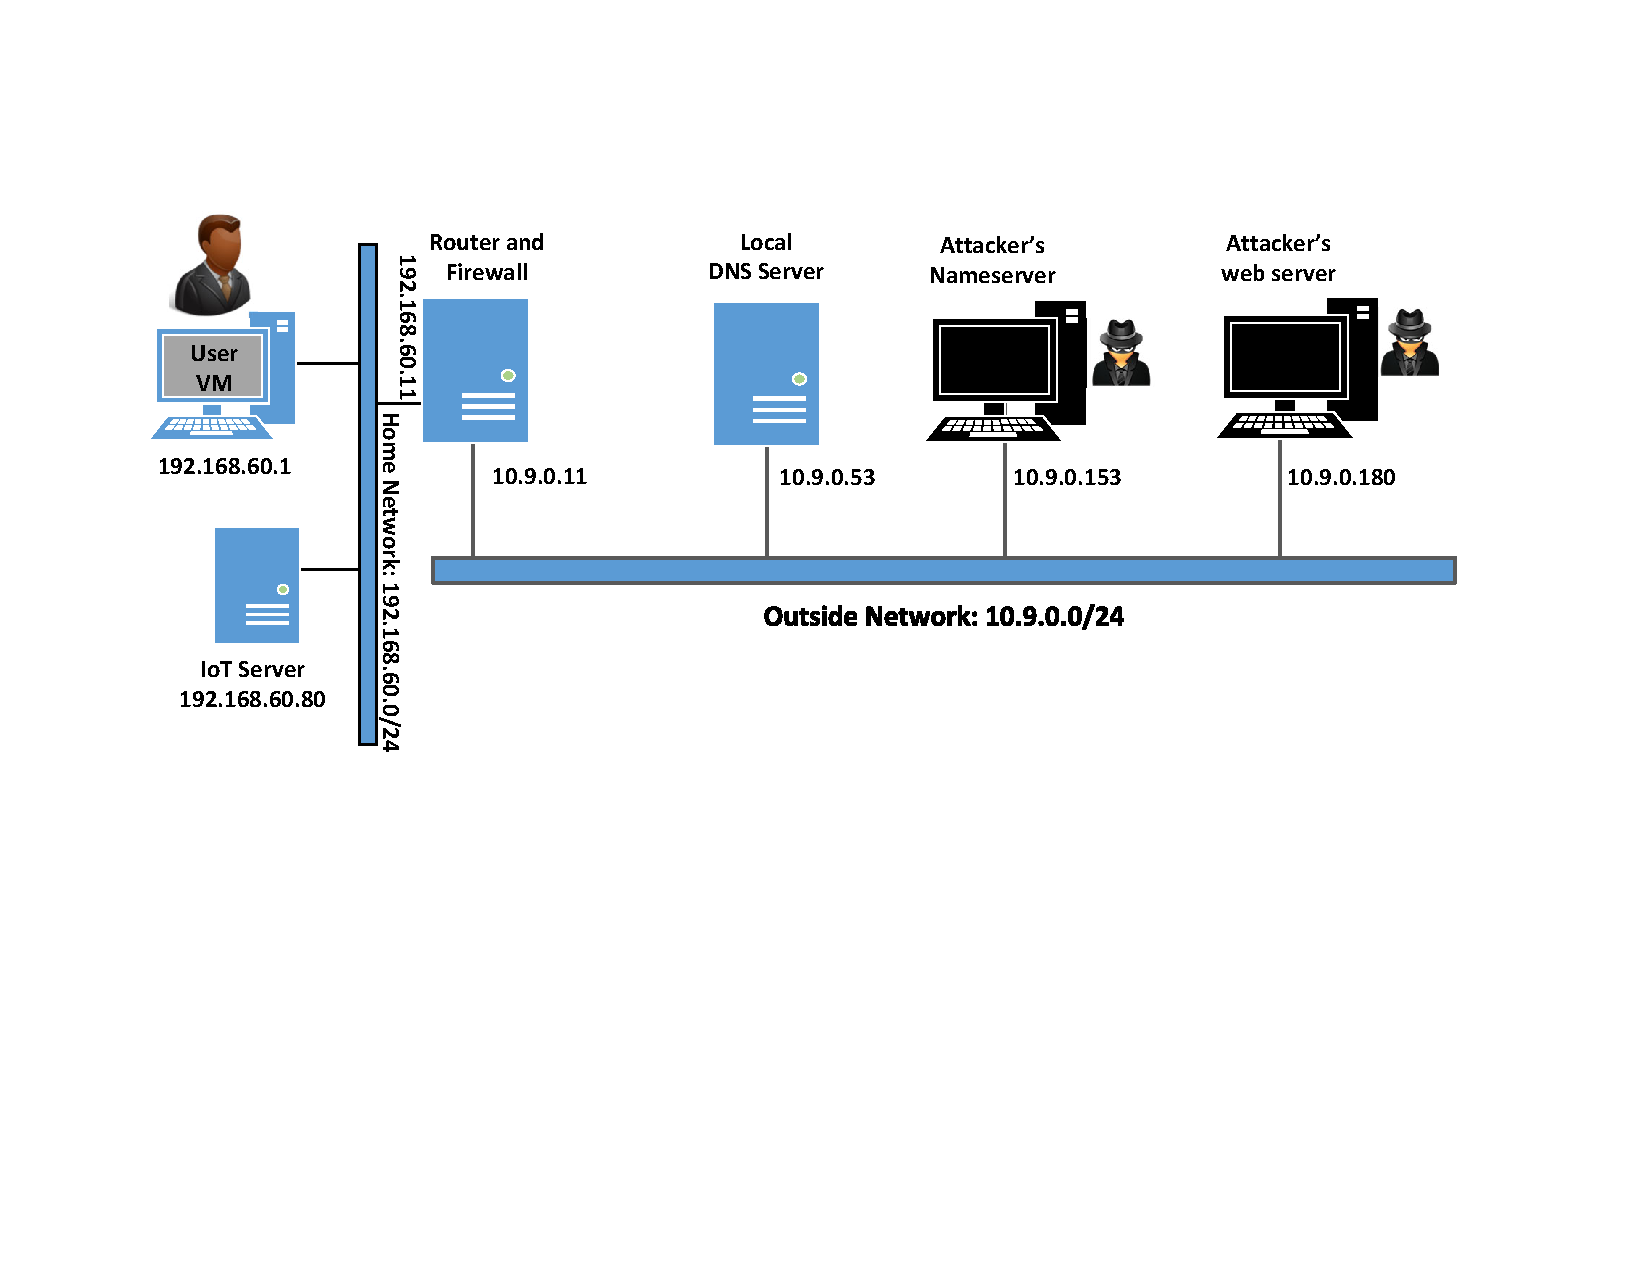
\includegraphics[width=0.9\textwidth]{\commonfolder/Figs/IoT_2lans.pdf}
\caption{Lab environment setup}
\label{rebind:fig:labsetup}
\end{figure}

En este laboratorio, usaremos seis máquinas.
El setup del entorno del entorno de laboratorio es ilustrado en la Figura \ref{rebind:fig:labsetup}. Sólo la máquina del usuario será una Máquina Virtual, el resto serán contenedores.
En el setup, tenemos dos redes, una red hogareña y otra red externa. La red hogareña simula una red típica de una casa. La máquina de usuario y el los servicios IoT están conectados a esta red, que es protegida por un firewall en un contenedor router. El firewall bloquea todo el tráfico  a \texttt{192.168.60.80}. De esta forma, las máquinas externas no pueden acceder al dispositivo.
También hemos un setup para un servidor NAT en el router, de esta forma las maquinas en la red hogareña pueden salir a Internet.

La segunda red simula el mundo externo. Aparte del router, existen tres contenedores conectados a esta red, uno es el servidor de DNS local, y los otros dos serán el nameserver de ataque y el web server.
El atacante posee el dominio \texttt{attacker32.com}, que está hosteado en el contenedor del nameserver. El web server hostea el sitio malicioso que es usado para el ataque.


% -------------------------------------------
% SUBSECTION
% -------------------------------------------
\subsection{Setup del Contenedor y sus Comandos}


%%%%%%%%%%%%%%%%%%%%%%%%%%%%%%%%%%%%%%%%%%%%
Para empezar a preparar el contenedor, deberá descargarse el archivo \texttt{Labsetup.zip} ubicado en el laboratorio correspondiente dentro del sitio web oficial y copiarlo dentro de la Máquina Virtual prevista por SEED. Una vez descargado deberá descomprimirlo y entrar dentro del directorio \texttt{Labsetup} donde encontrará el archivo \texttt{docker-compose.yml} que servirá para setear el entorno de laboratorio. Para una información más detallada sobre el archivo \texttt{Dockerfile} y otros archivos relacionados, puede encontrarla dentro del Manual de Usuario del laboratorio en uso, en el sitio web oficial de SEED.

Si esta es su primera experiencia haciendo el setup del laboratorio usando contenedores es recomendable que lea el manual anteriormente mencionado.

A continuación, se muestran los comandos más usados en Docker y Compose.
Debido a que estos comandos serán usados con mucha frecuencia, hemos creados un conjunto de alias para los mismos, ubicados en del archivo \texttt{.bashrc} dentro de la Máquina Virtual provista por SEED (Ubuntu 20.04)

\begin{lstlisting}
$ docker-compose build  # Build the container image
$ docker-compose up     # Start the container
$ docker-compose down   # Shut down the container

// Aliases for the Compose commands above
$ dcbuild       # Alias for: docker-compose build
$ dcup          # Alias for: docker-compose up
$ dcdown        # Alias for: docker-compose down
\end{lstlisting}


Dado que todos los contenedores estarán corriendo en un segundo plano. Necesitamos correr comandos para interactuar con los mismos, una de las operaciones fundamentales es obtener una shell en el contenedor. 
Para este propósito usaremos \texttt{"docker ps"} para encontrar el ID del contenedor deseado y ingresaremos \texttt{"docker exec"} para correr una shell en ese contenedor.
Hemos creado un alias para ello dentro del archivo \texttt{.bashrc}

\begin{lstlisting}
$ dockps        // Alias for: docker ps --format "{{.ID}}  {{.Names}}" 
$ docksh <id>   // Alias for: docker exec -it <id> /bin/bash

// The following example shows how to get a shell inside hostC
$ dockps
b1004832e275  hostA-10.9.0.5
0af4ea7a3e2e  hostB-10.9.0.6
9652715c8e0a  hostC-10.9.0.7

$ docksh 96
root@9652715c8e0a:/#  

// Note: If a docker command requires a container ID, you do not need to 
//       type the entire ID string. Typing the first few characters will 
//       be sufficient, as long as they are unique among all the containers. 
\end{lstlisting}

En caso de problemas configurando el entorno, por favor consulte la sección ``Common Problems'' en el manual ofrecido por SEED. 


%%%%%%%%%%%%%%%%%%%%%%%%%%%%%%%%%%%%%%%%%%%%



% -------------------------------------------
% SUBSECTION
% ------------------------------------------- 
\subsection{Configurar la Máquina Virtual del Usuario}

Necesitamos proporcionar una configuración adicional en la máquina virtual del usuario.


\paragraph{Paso 1.Reducir el tiempo de expiración de la caché DNS del Firefox.}
Con el objetivo de reducir la carga en los servidores DNS y optimizar los tiempos de respuestas, el navegador Firefox cachea los resultados de los DNS. Por defecto el tiempo de expiración de esta caché es de 60 segundos. Eso quiere decir que nuestro ataque de DNS Rebinding necesita esperar al menos 60 segundos. Para hacer todo mas sencillo, hemos reducido este tiempo a 10 segundos o menos. Para esto en la barra de navegación escriba  \texttt{about:config}. 
Despues de hacer click y pasar la página de advertencia, veremos una lista de preferencias con sus nombres y valores correspondientes.
Busque \texttt{dnsCache} encuentre la entrada y cambie su valor:

\begin{lstlisting}
(*@\textbf{network.dnsCacheExpiration}@*): cambie el valor a 10 (el valor por defecto es 60)
\end{lstlisting}

Después de hacer este cambio, debe de reiniciar el navegador, de otra forma no tomará efecto.


\paragraph{Paso 2. Cambiar \texttt{/etc/hosts}.}
Necesitamos agregar la siguiente entrada en el archivo \texttt{/etc/hosts}. Usaremos \texttt{www.seedIoT32.com} como el nombre para el servidor IoT. Su dirección IP es \texttt{192.168.60.80}. 
Necesitamos tener privilegios de superusuario para modificar este archivo (usando \texttt{sudo}): 

\begin{lstlisting}
192.168.60.80  www.seedIoT32.com
\end{lstlisting}

Mientras este editando este archivo, verifique si existe alguna entrada que contenga \texttt{attacker32.com}. Si está presente borrela.

Estamos listos para testear el servidor IoT. Ingreser en su navegador la siguiente URL usando la máquina virtual de usuario. Si está todo configurado correctamente, deberíamos de ver un termostato. También podemos cambiar la temperatura usando la barra de sliding. Por favor provea una captura de pantalla en su informe de laboratorio.

\begin{lstlisting}
http://www.seedIoT32.com
\end{lstlisting}
 

\paragraph{Paso 3. Servidor de DNS local.}
Necesitamos que la máquina virtual del usuario use un servidor de DNS local particular.
Esto se logra cambiando el archivo de configuración (\texttt{/etc/resolv.conf}) en la máquina del usuario de manera tal que se agregará la dirección IP del contenedor como la primera entrada \texttt{nameserver} dentro de este archivo, es decir, este servidor será usado como el servidor de DNS primario.
Desafortunadamente nuestra Máquina Virtual usa DHCP para obtener los parámetros de la configuración de red, tales como la dirección IP, el servidor de DNS local, etc. Los clientes DHCP sobreescribirán el archivo \texttt{/etc/resolv.conf} con su la información provista por el servidor DHCP.

Una forma de evitar esto es agregar la siguiente entrada dentro del archivo \path{/etc/resolvconf/resolv.conf.d/head}  (\texttt{10.9.0.53} es la dirección IP de nuestro servidor de DNS local que hemos configurado en el setup):

\begin{lstlisting}
nameserver 10.9.0.53
\end{lstlisting}

El contenido del archivo head será antepuesto al que se usa en la generación dinámica por el DHCP. Después de hacer este cambio necesitamos correr el siguiente comando para que tome efecto.

\begin{lstlisting}
$ sudo resolvconf -u
\end{lstlisting}




% -------------------------------------------
% SUBSECTION
% ------------------------------------------- 
\subsection{Probando el Setup del Laboratorio.}

Después de configura la máquina virtual del usuario, use el comando \texttt{dig} para obtener la dirección IP de \texttt{www.attacker32.com} y \texttt{ns.attacker32.com}. Debería de obtener \texttt{10.9.0.180} y \texttt{10.9.0.153} respectivamente. Si ud. no obtiene estas direcciones su entorno de laboratorio no fue configurado correctamente.

Ahora podemos testear el sitio del atacante.
Ingrese la siguiente URL en la máquina virtual del usuario y debería de poder ingresar al sitio del atacante.
Por favor incluya una captura de pantalla en su informe de laboratorio.


\begin{lstlisting}
http://www.attacker32.com
\end{lstlisting}

\paragraph{Note.} We may have used the same hostname  
\texttt{www.attacker32.com} in other SEED labs, so it is likely 
that this name is already mapped to a different IP address. Therefore,
if you do not see the expected attacker's website, you should 
check the \texttt{/etc/hosts} file, and remove
any entry that contains \texttt{attacker32.com}. 




% *******************************************
% SECTION
% ******************************************* 
\section{Lanzando el Ataque en el Dispositivo IoT}

Estamos listos para lanzar el ataque en el dispositivo IoT. Para una mejor comprensión de parte de los estudiantes en como funciona el ataque, hemos fragmentado el ataque en varios pasos incrementales.


% -------------------------------------------
% SUBSECTION
% ------------------------------------------- 
\subsection{Tarea 1. Entendiendo la Protección de Same-Origin Policy}

In this task, we will do some experiment to understand the 
same-origin policy protection implemented on browsers. On the user VM,
we will browse the following three URLs. It is better to show these three pages on three
different Firefox windows (instead of on three different tabs), so they are all visible. 


\begin{lstlisting}
URL 1:  http://www.seedIoT32.com
URL 2:  http://www.seedIoT32.com/change
URL 3:  http://www.attacker32.com/change
\end{lstlisting}

 
The first page lets us see the current temperature setting of the thermostat (see
Figure~\ref{rebinding:fig:webpages}.a); it fetches
the temperature value from the IoT server once every second. We should keep this page always
visible, so we can see the temperature setting on the thermostat. 
The second and third pages
are identical (see Figure~\ref{rebinding:fig:webpages}.b), 
except that one comes from the IoT server, and the other comes from
the attacker's server. When we click the button on both pages, 
a request will be sent out to the IoT server to set its temperature. 
We are supposed to raise the thermostat's temperature 
to \texttt{99} Celsius.  


\begin{figure}[htb]
\begin{center}
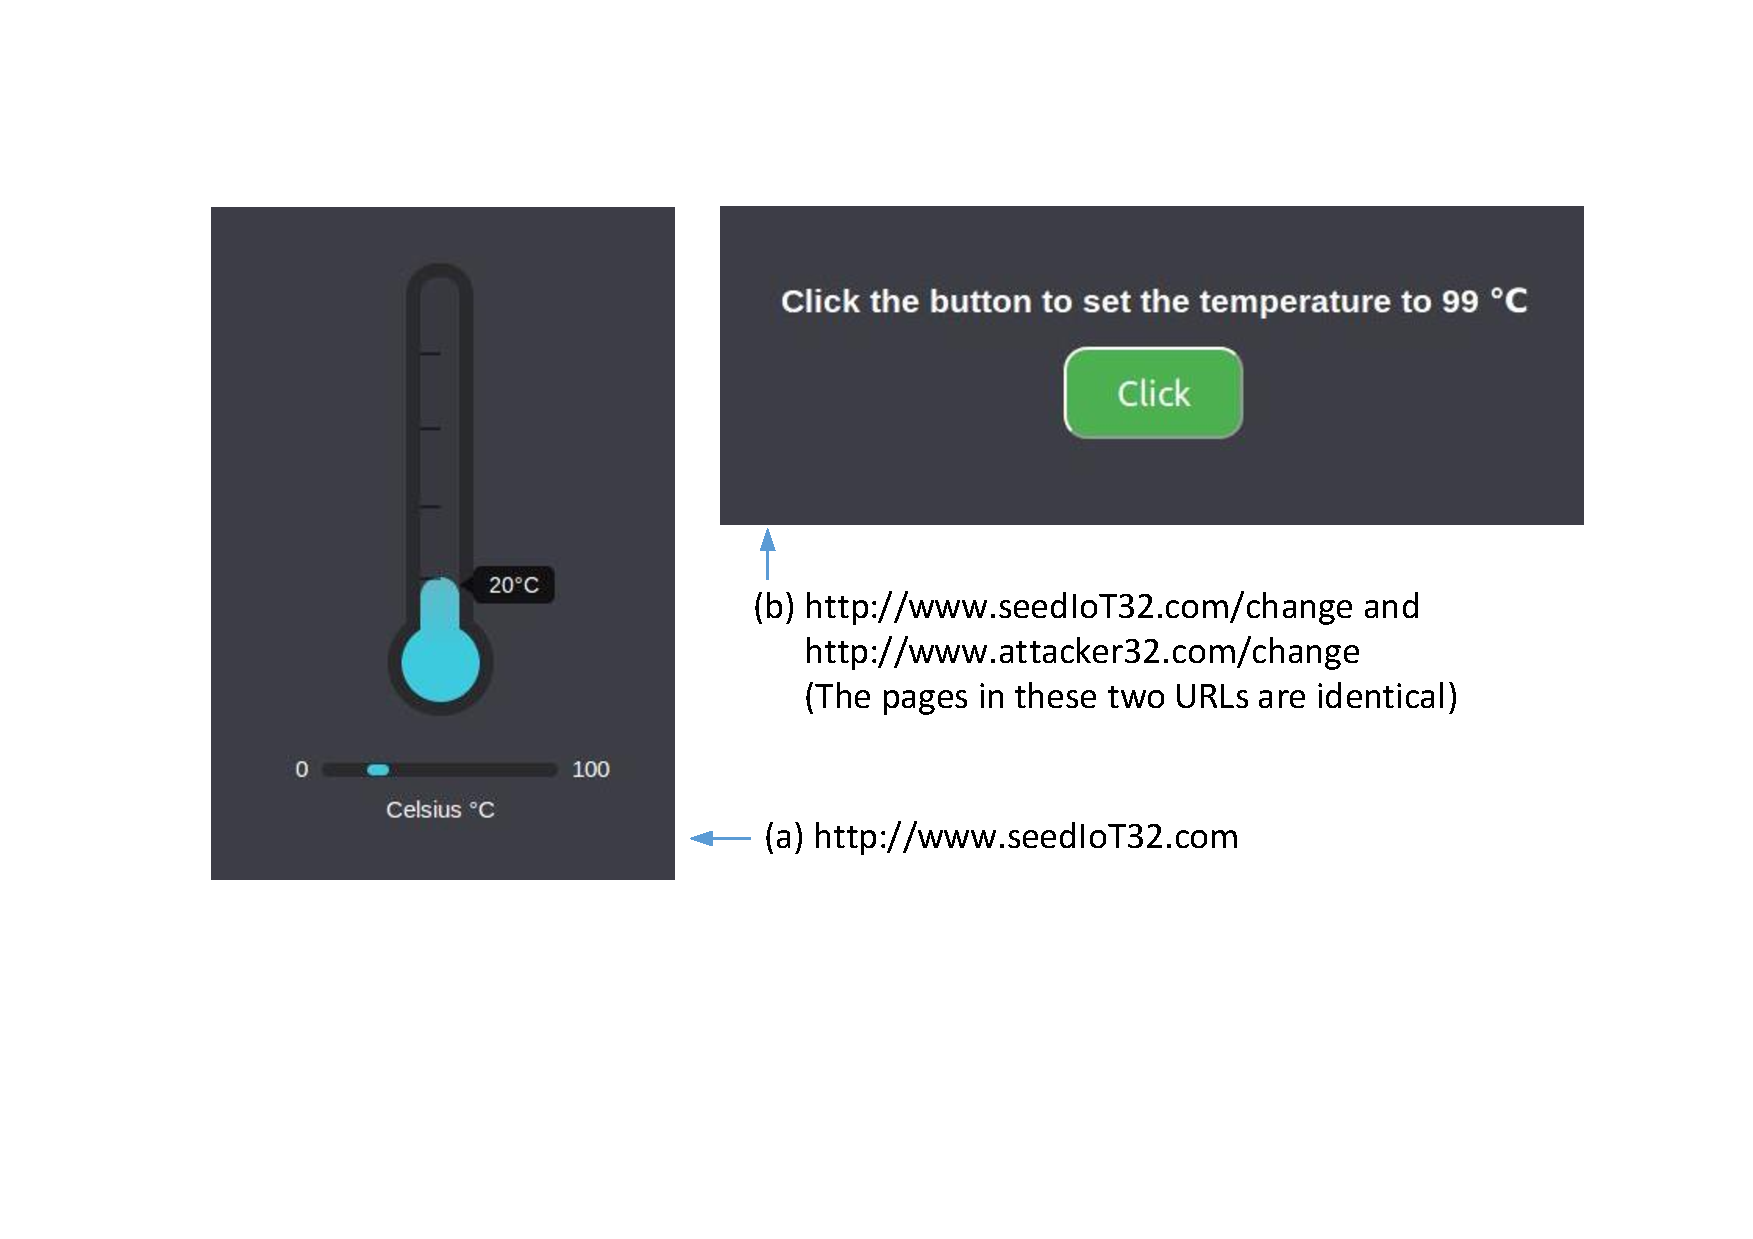
\includegraphics[width=0.8\textwidth]{\rebindingFigs/iot_webpages.pdf}
\end{center}
\caption{The web pages from the three URLs}
\label{rebinding:fig:webpages}
\end{figure}
 

Click the button on the second and third pages, and describe your observation. Which page
can successfully set the thermostat's temperature? Please explain why. 
To find the reason, click the following menu sequence from Firefox. A console window will appear,
which displays error messages if any. Hint: the reason is related to the same-origin policy 
enforced by browsers. Please explain why this policy causes one of the pages to fail.
 
\begin{lstlisting}
Web Developer -> Web Console
\end{lstlisting}
  


% -------------------------------------------
% SUBSECTION
% ------------------------------------------- 
\subsection{Task 2. Defeat the Same-Origin Policy Protection}


From the previous task, it seems impossible to
set the thermostat's temperature from the attacker's
page, due to the browser's   
same-origin policy protection.  The objective of this task
is to defeat such a protection, so we can set the 
temperature from this page. 


The main idea for defeating the same origin protection 
comes from the fact that the policy enforcement is 
based on the host name, not on the IP address, so as long as 
we use \texttt{www.attacker32.com} in the URL, we are complying with
the SOP policy, but that does not mean we are restricted 
to communicate with the \texttt{www.attacker32.com} web server.  


Before the user's browser sends out requests to \texttt{www.attacker32.com},
it first needs to know the IP address of \texttt{www.attacker32.com}. 
A DNS request will be sent out from the user's machine. If the 
IP address is not cached at the local DNS server, a DNS request will
eventually be sent to \texttt{attacker32.com}'s  nameserver, which 
is controlled by the attacker. 
Therefore, the attacker can decide what to put in the response. 


\paragraph{Step 1: Modify the JavaScript code.}
On the attacker's web server, the JavaScript code running inside the 
\url{www.attacker32.com/change} page is 
stored in the following file: 
\path{/app/rebind_server/templates/js/change.js}. Since this page
comes from the \texttt{www.attacker32.com} server, 
according to the same-origin policy, it can only
interact with the same server. Therefore, we need to change the first 
line of the code from \url{http://www.seediot32.com} 
to the following (we have installed a simple editor called \texttt{nano}
in the container):

\begin{lstlisting}
let url_prefix = 'http://www.attacker32.com'
\end{lstlisting}
 

After making the change, restart the attacker's web server container (see the 
command below). Then go to the user VM, refresh the page, and click the button again. 
Do you still see the error
message in the web console? Please explain your observation. 


\begin{lstlisting}
$ docker ps
...
78359039627a  attacker-www-10.9.0.180

$ docker container restart 7835
\end{lstlisting}
 


\paragraph{Step 2: Conduct the DNS rebinding.}
Our JavaScript code sends requests to \url{www.attacker32.com}, 
i.e., the requests will come back to the Attacker's web server. That is not 
what we want; we want the requests to go to the IoT server. 
This can be achieved using the DNS rebinding 
technique. We first map \url{www.attacker32.com} to the IP address of the attacker's
web server, so
the user can get the actual page from \url{http://www.attacker32.com/change}. 
Before we click on the button on the page, we remap
the \url{www.attacker32.com} hostname to the IP address of the IoT server, so
the request triggered by the button will go to the IoT server. That is exactly what 
we want. 


To change the DNS mapping, students can modify the 
\path{zone_attacker32.com} file inside attacker's nameserver container.
The zone file can be found in 
the \texttt{/etc/bind} folder. 
The following shows the content of the zone file. The first 
entry is the default Time-To-Live (\texttt{TTL}) value (seconds) 
for the response, specifying how long the response can stay in
the DNS cache. This value may need to be modified. 
The following is the content of the zone file:

\begin{lstlisting}
$TTL 1000
@       IN      SOA   ns.attacker32.com. admin.attacker32.com. (
                2008111001
                8H
                2H
                4W
                1D)

@       IN      NS    ns.attacker32.com.

@       IN      A     10.9.0.22
www     IN      A     10.9.0.22
ns      IN      A     10.9.0.21
*       IN      A     10.9.0.22
\end{lstlisting}


After making the changes to the zone file, 
run the following command to ask the nameserver 
to reload the revised zone data. 

\begin{lstlisting}
# rndc reload attacker32.com
\end{lstlisting}



Because of the tasks conducted previously, the DNS mapping for the 
\texttt{www.attacker32.com} has already been cached by the local
DNS server, it will not expire until 1000 seconds later.  To 
shorten the waiting, students are allowed to clean out the cache using the 
following command (on the local DNS server). However, this can only be 
conducted before the attack starts. Once the attack starts, students 
are not allowed to touch the local DNS server. 

\begin{lstlisting}
// Do it on the local DNS server container
# rndc flush
\end{lstlisting}
 
 
If both steps in this task are done correctly, clicking the button 
on the \texttt{change} page from \url{www.attacker32.com} should be able to change
the thermostat's temperature successfully. Please provide evidence in your report to
demonstrate your success.


% -------------------------------------------
% SUBSECTION
% ------------------------------------------- 
\subsection{Task 3. Launch the Attack}

In the previous task, the user has to click the button to set the 
temperature to the dangerously high value. Obviously, it is unlikely that users will 
do that.  In this task, we need to do that automatically. We have already created 
a web page for that purpose. It can be accessed using the following URL:


\begin{lstlisting}
http://www.attacker32.com
\end{lstlisting}
 

Once you have loaded this page into the user VM, you should be able to see a page with a 
timer, which goes down from 10 to 0. Once it reaches 0, the JavaScript code 
on this page will send the set-temperature request to 
\url{http://www.attacker32.com}, and then reset the timer value to 10. 
Students need to use the DNS rebinding technique, so
once the timer reaches 0, the thermostat's temperature is set to 
88 Celsius. 



% *******************************************
% SECTION
% *******************************************
\section{Informe del Laboratorio}

%%%%%%%%%%%%%%%%%%%%%%%%%%%%%%%%%%%%%%%%

Debe enviar un informe de laboratorio detallado, con capturas de pantalla, para describir lo que ha hecho y lo que ha observado.
También debe proporcionar una explicación a las observaciones que sean interesantes o sorprendentes.
Enumere también los fragmentos de código más importantes seguidos de una explicación. No recibirán créditos aquellos fragmentos de códigos que no sean explicados.
%%%%%%%%%%%%%%%%%%%%%%%%%%%%%%%%%%%%%%%%

\section*{Agradecimientos}

Este documento ha sido traducido al Español por Facundo Fontana




\end{document}
